\documentclass[tikz,border=10pt]{standalone}
\usepackage[T1]{fontenc}
\usepackage{lmodern}
\usetikzlibrary{arrows.meta}
\definecolor{ink}{HTML}{183444}
\definecolor{blue}{HTML}{1B6780}
\definecolor{amber}{HTML}{AD601A}
\begin{document}
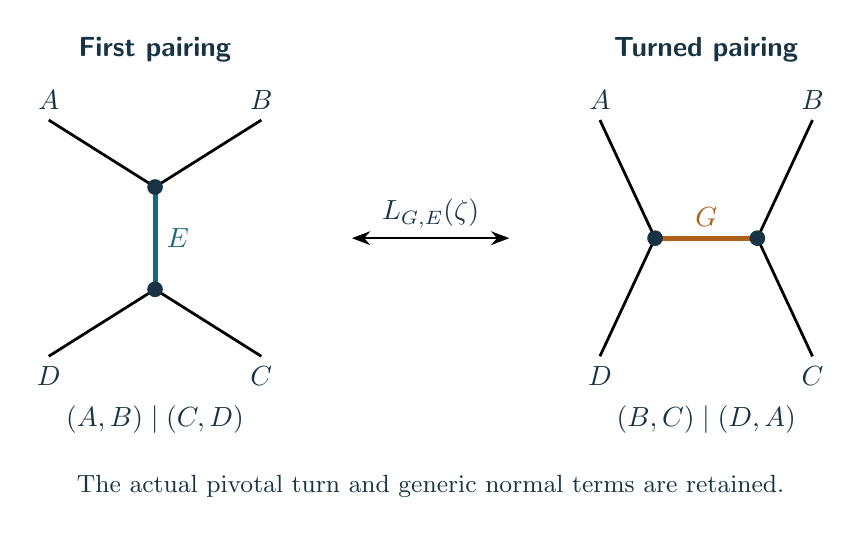
\begin{tikzpicture}[font=\sffamily,text=ink,line width=1pt,vertex/.style={circle,fill=ink,inner sep=2pt}]
 \begin{scope}[xshift=-3.5cm]
  \node at (0,2.4) {\textbf{First pairing}};
  \coordinate (t) at (0,.65);\coordinate (b) at (0,-.65);
  \draw (-1.35,1.5) node[above] {$A$}--(t)--(1.35,1.5) node[above] {$B$};
  \draw (-1.35,-1.5) node[below] {$D$}--(b)--(1.35,-1.5) node[below] {$C$};
  \draw[blue,line width=1.8pt] (t)--node[right] {$E$}(b);
  \node[vertex] at(t){};\node[vertex] at(b){};
  \node at(0,-2.3) {$(A,B)\mid(C,D)$};
 \end{scope}
 \draw[<->,>=Stealth,thick] (-1,0)--node[above] {$L_{G,E}(\zeta)$}(1,0);
 \begin{scope}[xshift=3.5cm]
  \node at (0,2.4) {\textbf{Turned pairing}};
  \coordinate(l)at(-.65,0);\coordinate(r)at(.65,0);
  \draw (-1.35,1.5) node[above] {$A$}--(l)--(-1.35,-1.5) node[below] {$D$};
  \draw (1.35,1.5) node[above] {$B$}--(r)--(1.35,-1.5) node[below] {$C$};
  \draw[amber,line width=1.8pt] (l)--node[above] {$G$}(r);
  \node[vertex] at(l){};\node[vertex] at(r){};
  \node at(0,-2.3) {$(B,C)\mid(D,A)$};
 \end{scope}
 \node[font=\small] at(0,-3.15) {The actual pivotal turn and generic normal terms are retained.};
\end{tikzpicture}
\end{document}
